\documentclass[]{auvsi_doc}
\setkeys{auvsi_doc.cls}{
	AUVSITitle={Unmanned Ground Vehicle Parachute Testing Description}
	%AUVSILogoPath={./logo.pdf]}
}

% include extra packages, if needed
\usepackage{longtable}
\usepackage{gensymb}
\usepackage{subcaption}


\begin{document}

\begin{AUVSITitlePage}
\begin{artifacttable}
\entry{GV-003, 0.1, 2018-10-30, Initial Draft, John Akagi, Kameron Eves}
\entry{GV-003, 1.0, 2018-11-6, Revised after design review, John Akagi, Andrew Torgesen}
\entry{GV-003, 1.1, 2018-11-8, Added Intro and Conclusion. Fixed minor errors, Brady Moon, ----}
% additional \entry{} commands for extra rows in the revision table, if needed
\end{artifacttable}
\end{AUVSITitlePage}

\section{Introduction}
This artifact details the methods and results of testing the selected UGV drop system concepts from GV-001.

\section{Testing}
The parachute concepts were tested in high bay in the Engineering Research Lab. There is scaffolding that allowed us an approximately 35 foot drop into a 20 foot by 10 foot area. Initial testing was done on the methods to measure the landing velocity of the payload and to get a basic understanding of what variables were important to control. After the initial testing, we decided to test a large parachute, a small parachute, and a small parachute with control fins on the payload since these seemed to have the largest impact on the precision of the drop and the landing speed. The large parachute was 48 inches in diameter with a 16 inch diameter spill hole. The small parachute was 30 inches in diameter with a 6 inch diameter spill hole. The fin design was comprised of two fins with a total surface area of 19.5 in\textsuperscript{2}.

We tested these three methods by dropping each one three times and recording the impact point to evaluate how well the drop system met the key success measure of airdrop accuracy. The payload weight for each drop was .711 kg.  During these drops, we controlled the position, shape, and orientation of the parachute to reduce any effects that would be caused by imperfections in the construction of our parachute. For the drop with the fins, the fins were both oriented at approximately a 45\degree angle relative to vertical and turned to the right to try and offset the leftward drift of the small parachute. The parachute and setup for the parachute connections are shown in Figure \ref{fig:combined}. The results of the test are shown in Table \ref{table:results} and the drop locations are shown in Figure \ref{fig:locations}.

For each drop, the parachute was held on two opposite side in a way to try and equalize the tension in each of the parachute cords. The payload was allowed to hang freely beneath the parachute although the parachute was not released until any twisting motion of the payload had been damped out. Each payload was released from approximately the same place which was determined by visually lining the payload up with a target placed on the ground. The parachute was released into still air and the position of the initial impact was recorded by an observer on the ground. If the payload impacted the wall before reaching the ground, the observer would extrapolate the ground impact location by estimating the lateral speed and height of impact. The average initial impact position and the standard deviation of the spread were calculated. Additionally, the average impact position and standard deviation were calculated for a 100 ft drop using a simple linear extrapolation. We assumed that the payload would drift approximately 3 times times as far in a 100 ft drop as it would in a 35 ft drop,  multiplied the landing distances by that factor, and recalculated the standard deviation. While the actual payload drop will likely be less accurate due to cross winds and being dropped with an initial lateral velocity, these tests are useful in determining the relative accuracy of various delivery systems in ideal conditions.

\begin{figure}[ht]
\centering
   \begin{subfigure}{0.49\linewidth} \centering
     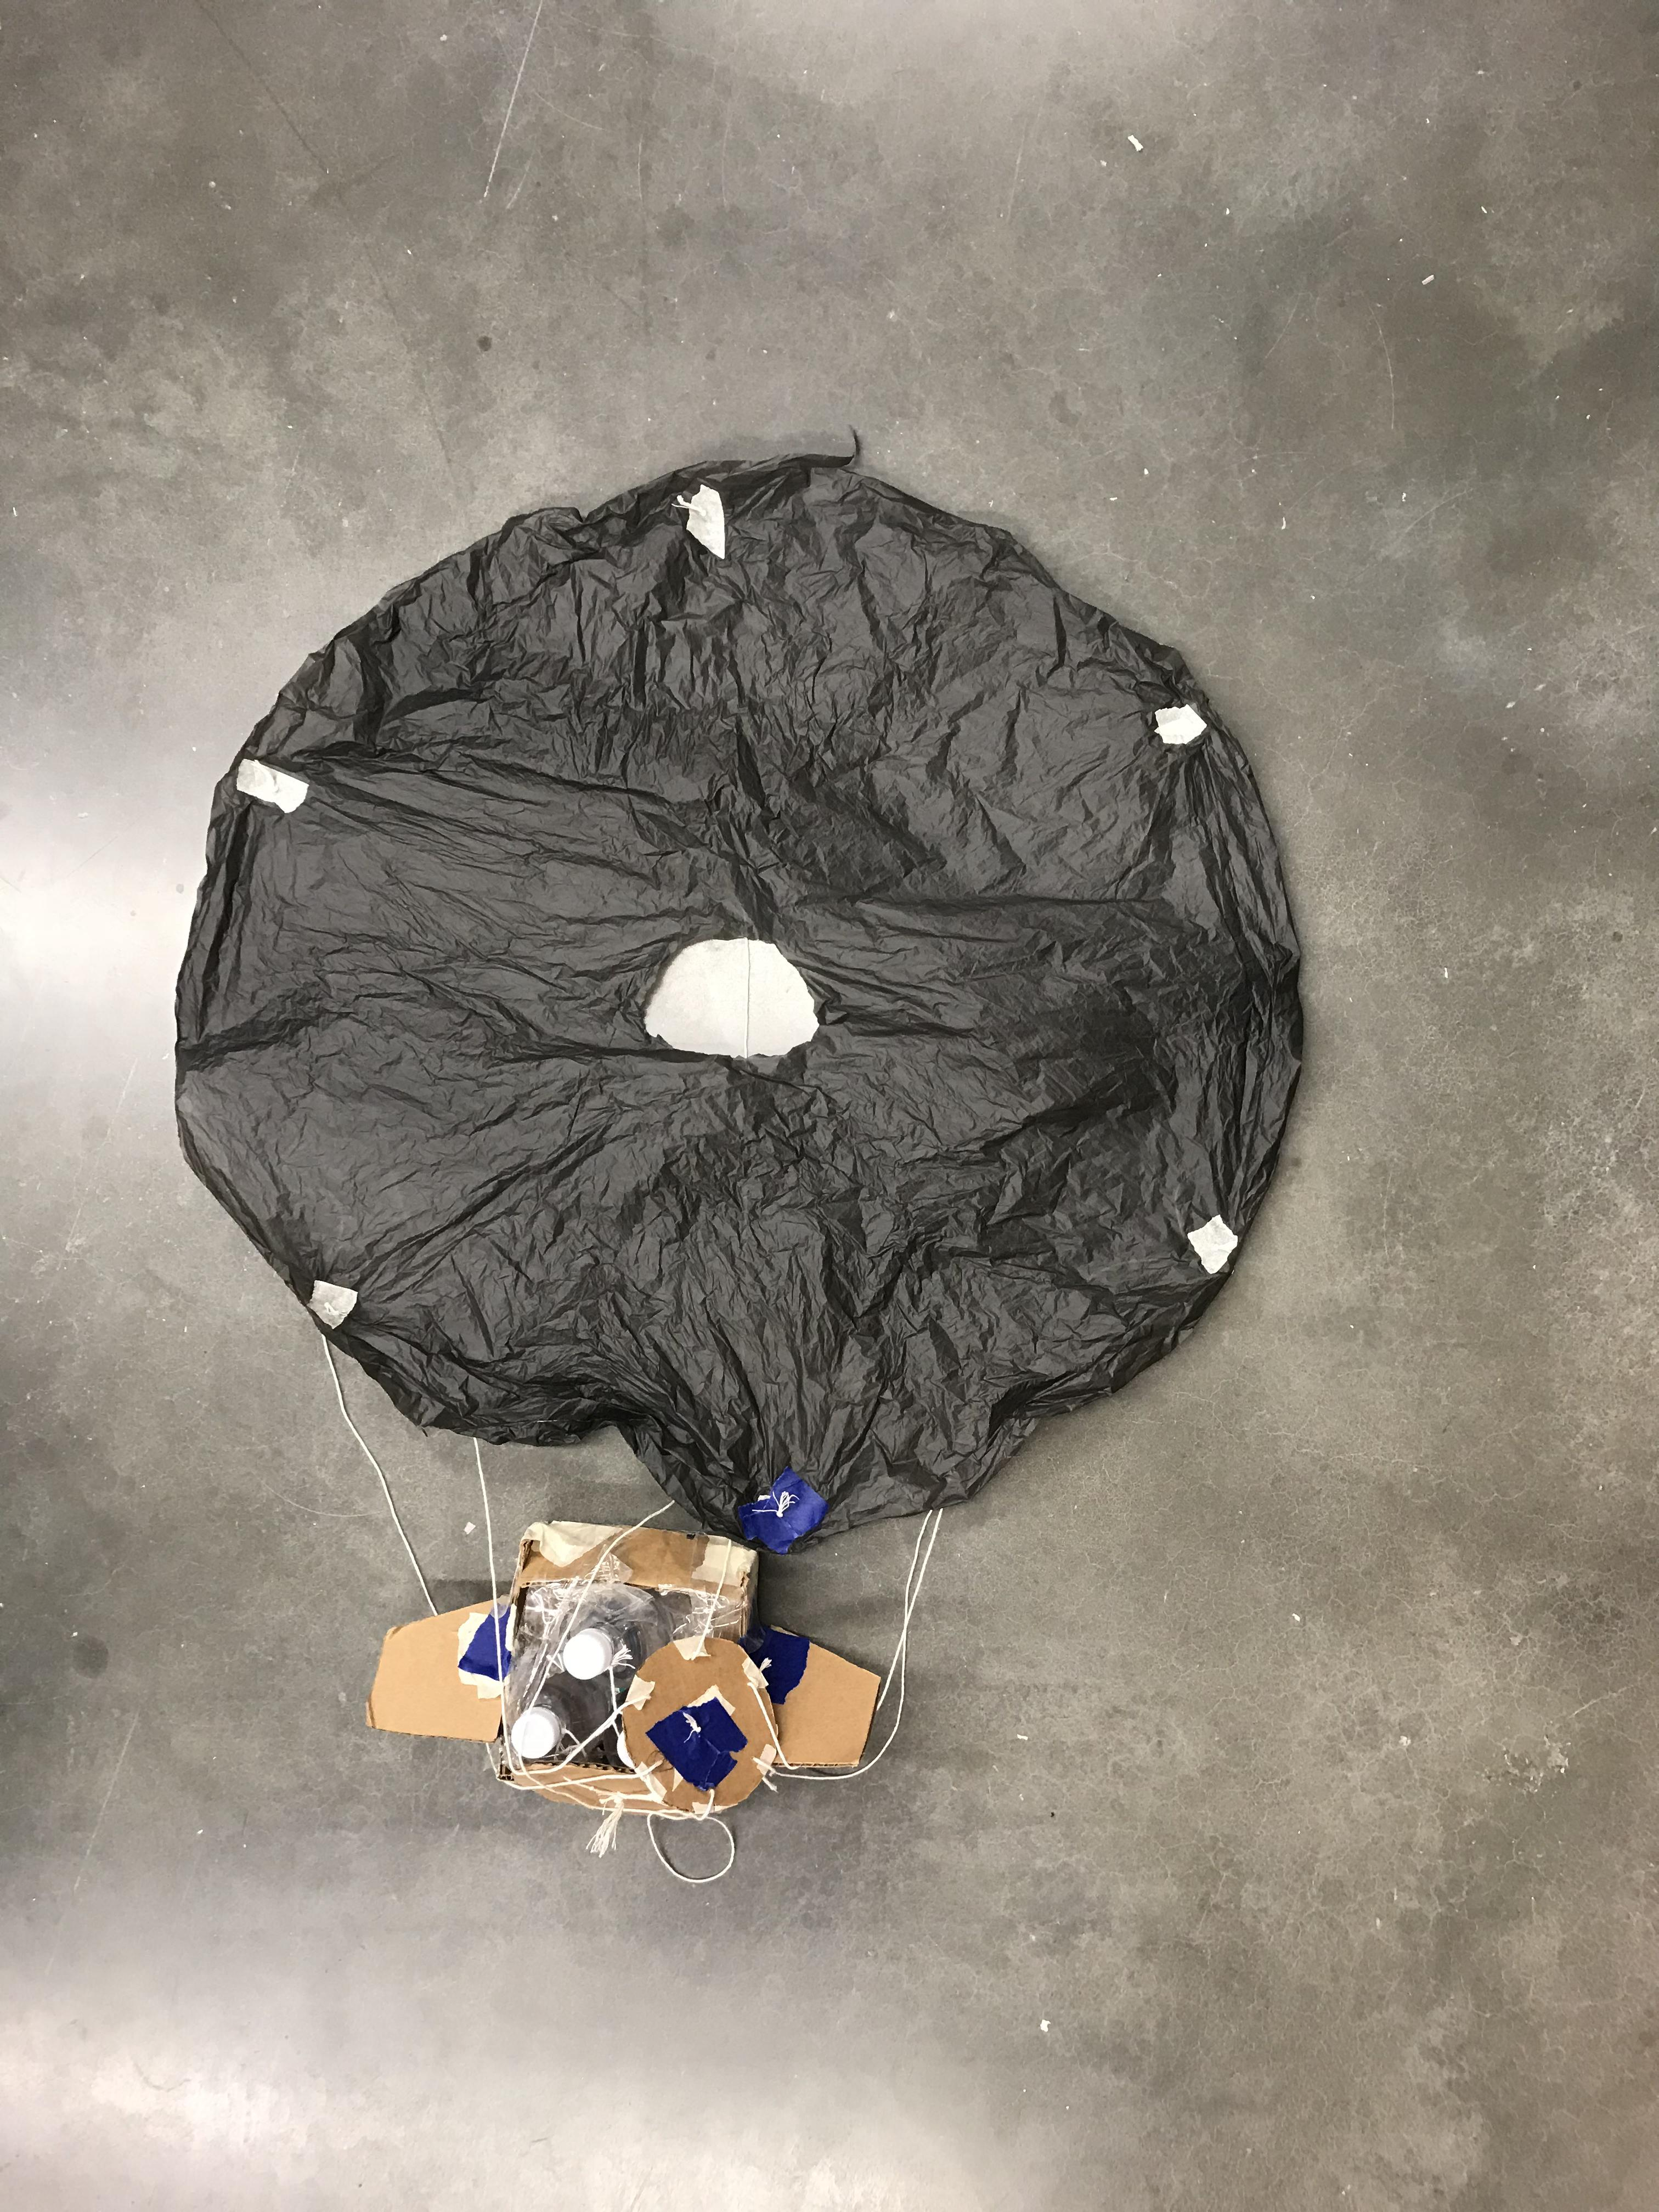
\includegraphics[width=.95\columnwidth]{Parachute1.jpg}
     \caption{Full configuration for parachute and fins.}\label{fig:fullParachute}
   \end{subfigure}
   \begin{subfigure}{0.49\linewidth} \centering
     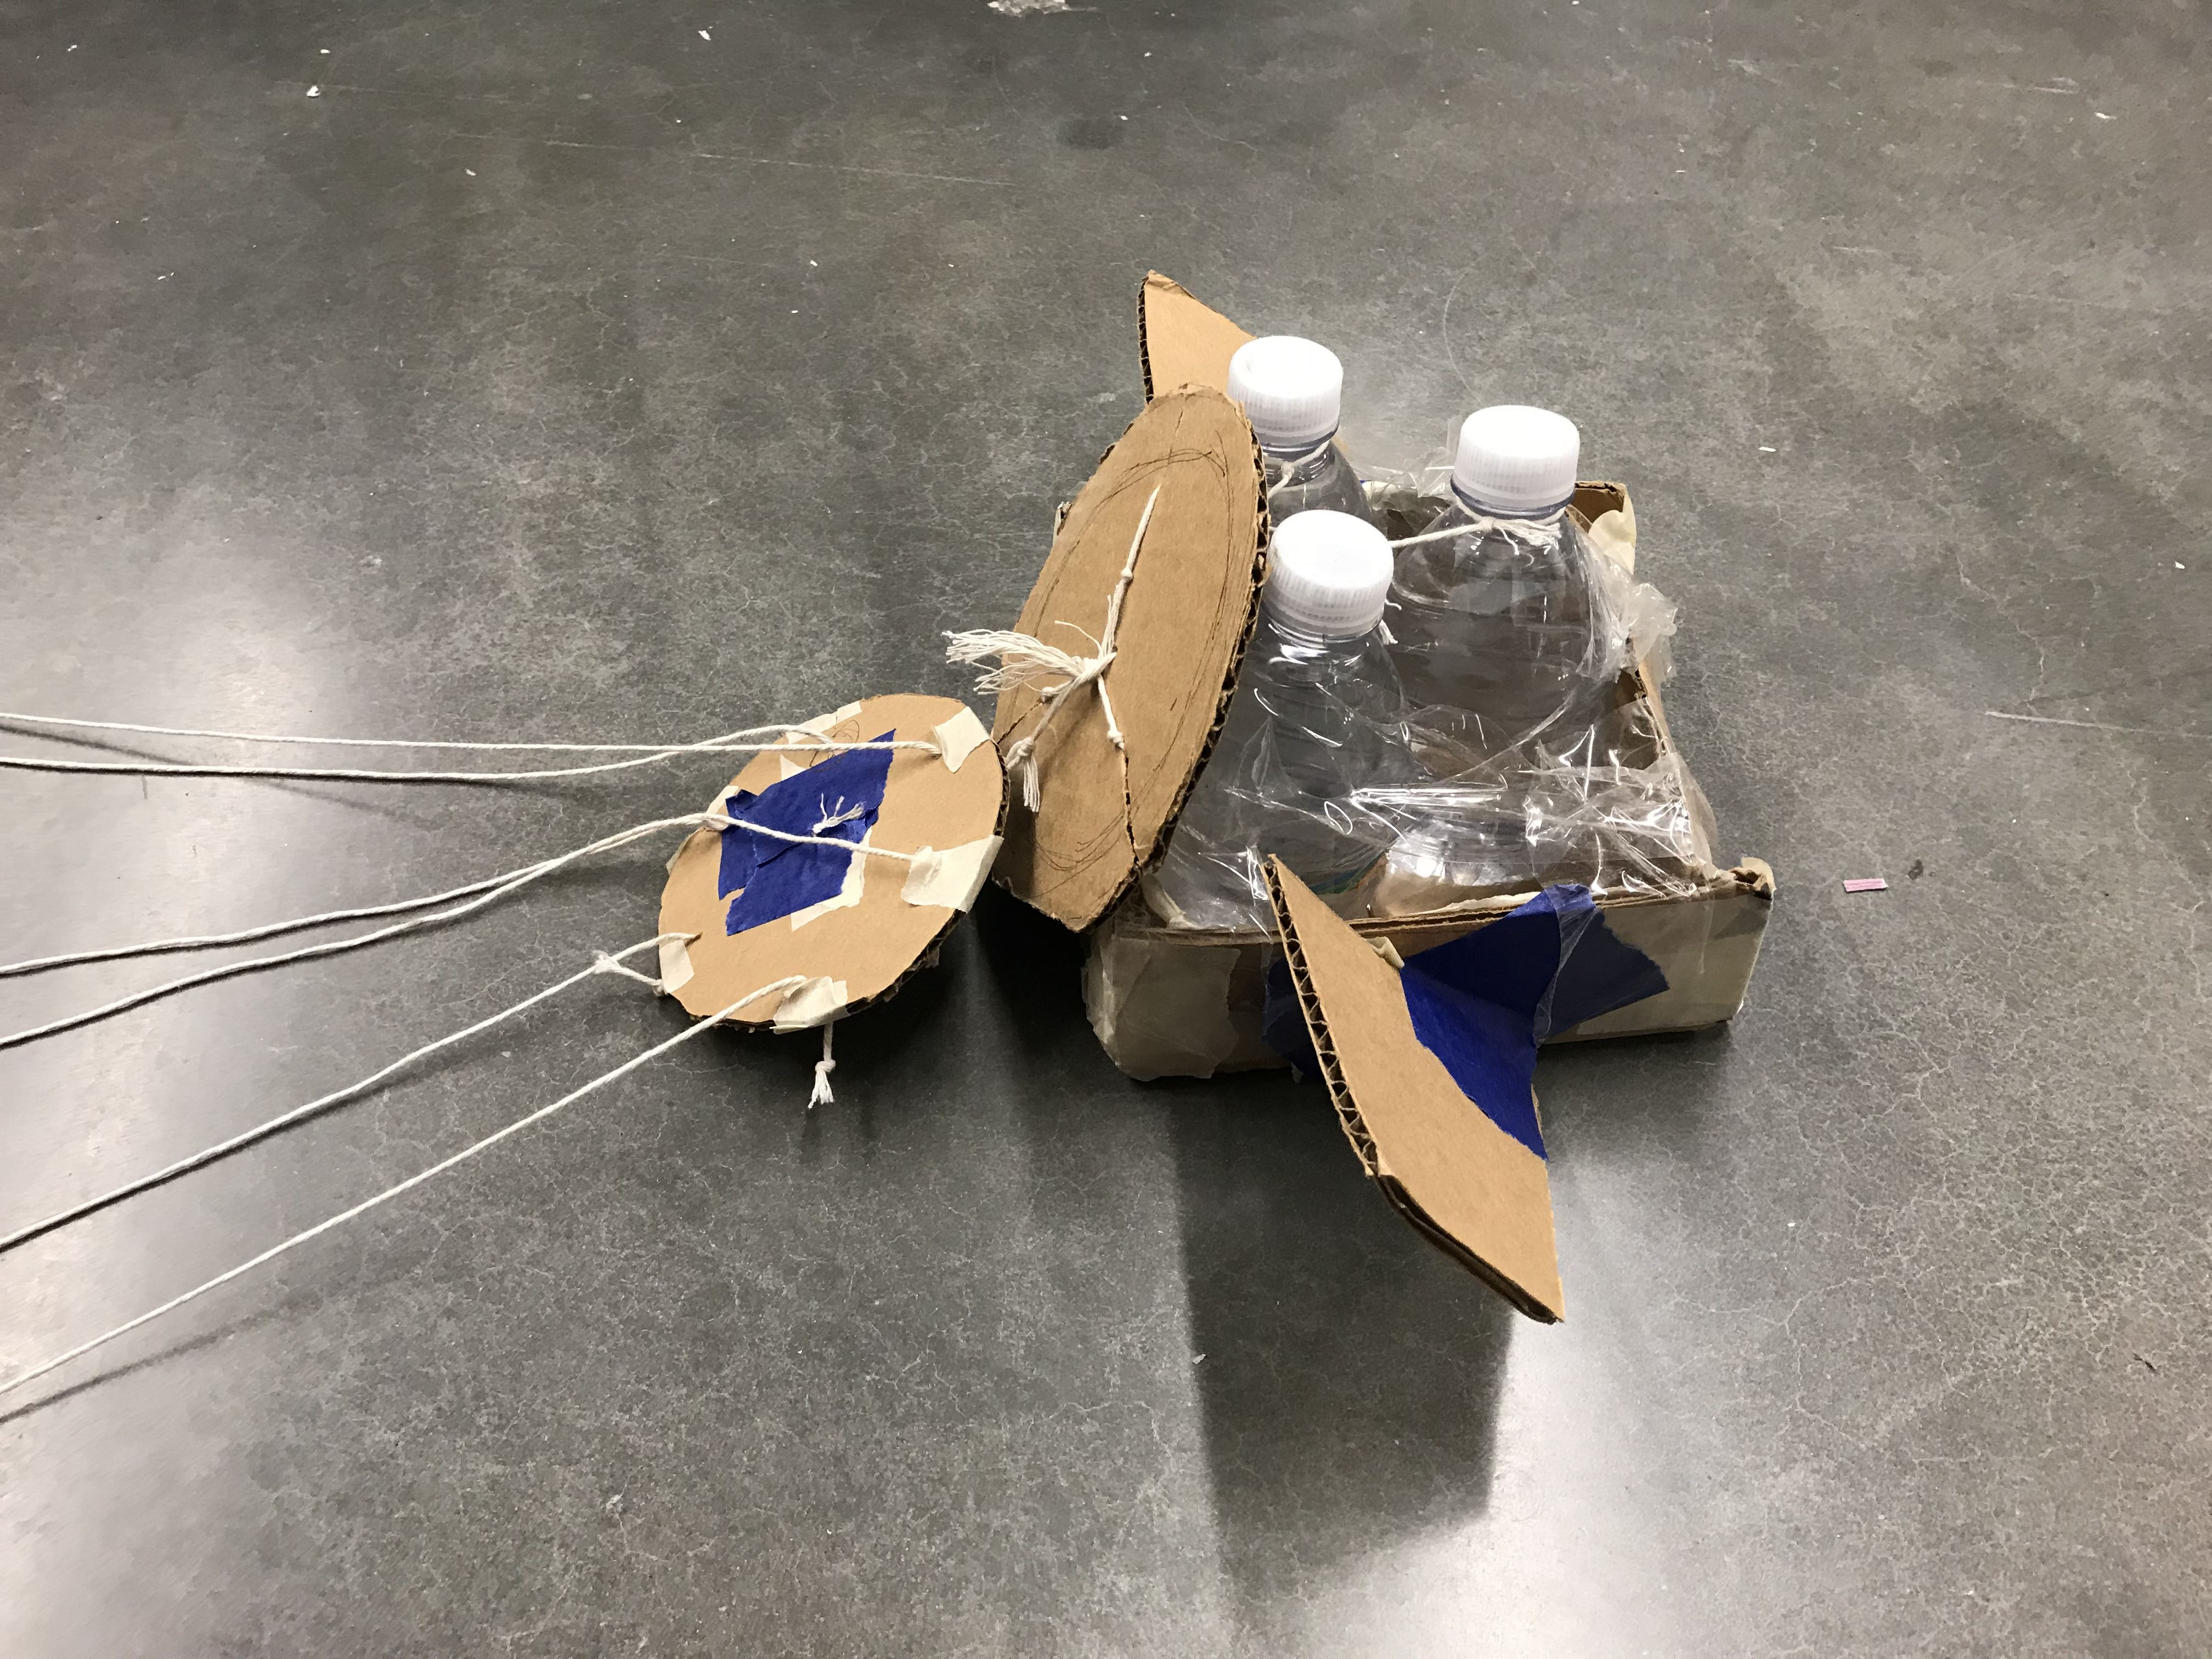
\includegraphics[width=.95\columnwidth]{Parachute2.jpg}
     \caption{Control fins and connections to parachute.}\label{fig:ControlFins}
   \end{subfigure}
\caption{Testing setup for the small parachute and fins option. The small parachute only method was the same but without the cardboard holder around the water bottles. The large parachute method was identical to the small parachute method but simply larger.}
\label{fig:combined}
\end{figure}

\begin{table}[h]
\caption{The results of dropping the three different parachute systems. The average distance is the average distance between the point directly below where the parachute was dropped and the initial landing spot. The standard deviation is the standard deviation between all three drops for each system. The scaled standard deviation is the estimated standard deviation when payloads are dropped from 100 ft. }
\label{table:results}

\begin{tabular}{| l | l | l | l |}
\hline
Method & Average Distance & Std. Deviation & Scaled Std. Dev.\\
\hline
Large Parachute & 9.01 ft  & 0.95 ft & 2.85 ft\\
Small Parachute & 7.20 ft  & 1.38 ft & 4.14 ft\\
Small Parachute with Fins & 4.70  & 1.08 ft & 3.23 ft\\
\hline

\end{tabular}

\end{table}

\begin{figure}[h]
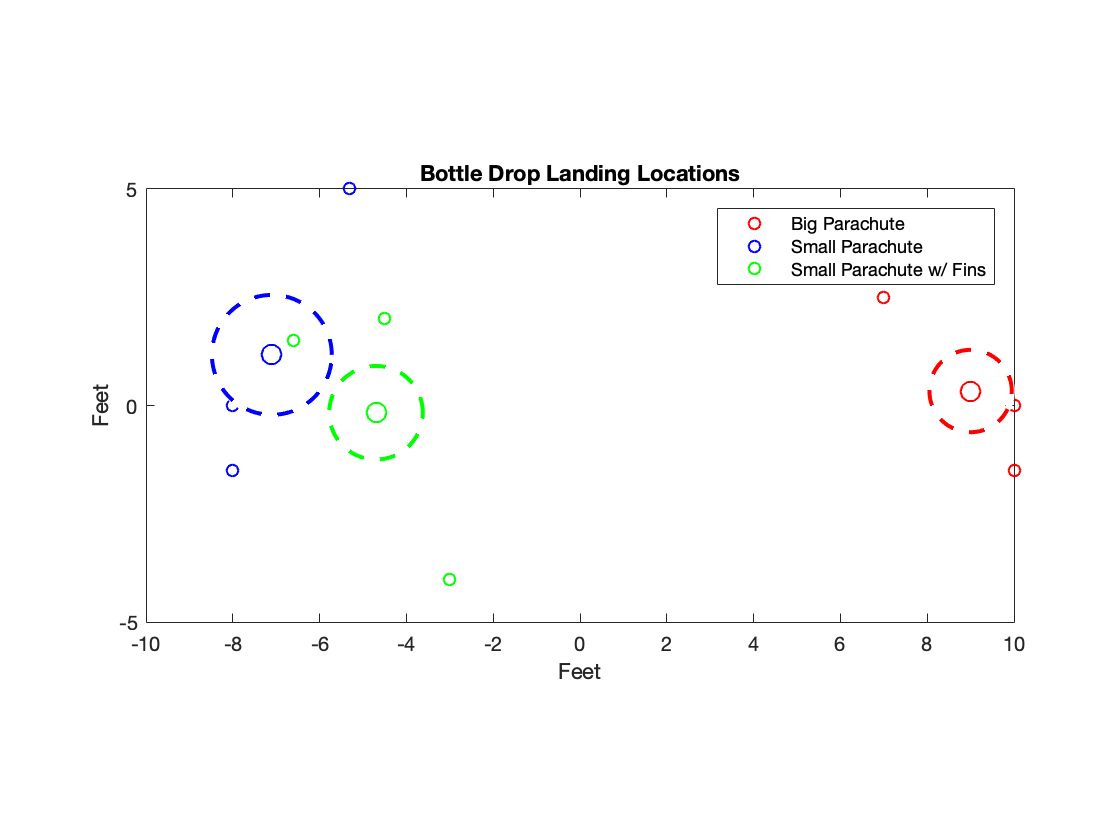
\includegraphics[width=\columnwidth]{LandingLocations.png}
\caption{The location of the initial impacts of each of the drops as shown by filled in circles. Due to the constrained area of our testing location, some landing locations were extrapolated since they hit the walls before the ground. The open circles are the average location of impact. The dashed lines indicate the mean distance away from the average impact location. The colors differentiate between system types as shown in the legend.}
\label{fig:locations}
\end{figure}

\section{Conclusion}
Test results are used in artifact GV-004 for overall comparison of our concepts.


\end{document}
